\documentclass[a4paper,9pt]{article}

\usepackage[a4paper, margin=0.55cm, top=0.4cm, bottom=0.35cm]{geometry}
\usepackage{graphicx}
\usepackage{xcolor}
\usepackage{multicol}
\usepackage{tcolorbox}
\usepackage{tikz}
\usetikzlibrary{positioning}
\usepackage[T1]{fontenc}
\usepackage[utf8]{inputenc}
\usepackage{parskip}
\usepackage{enumitem}
\usepackage{array}
\usepackage{booktabs}
\usepackage{float}
\usepackage{mdframed}

\tcbuselibrary{skins,breakable,fitting}

\definecolor{primary}{HTML}{00478C}
\definecolor{secondary}{HTML}{005BB3}
\definecolor{accent}{HTML}{0098FF}
\definecolor{lightbg}{HTML}{f4f9f6}
\definecolor{darkbg}{HTML}{00598F}
\definecolor{labeltext}{HTML}{000000}
\definecolor{textgray}{HTML}{3a3a3a}
\definecolor{tagbg}{HTML}{e6f2ec}

\newcommand{\sectiontitle}[1]{%
  \vspace{1pt}%
  {\color{primary}\rule{\linewidth}{1pt}}\\[-4pt]
  {\color{primary}\small\bfseries\MakeUppercase{#1}}\\[-8pt]
  {\color{secondary}\rule{\linewidth}{0.4pt}}%
  \vspace{2pt}%
}

\newlist{tightitem}{itemize}{1}
\setlist[tightitem]{leftmargin=*,noitemsep,topsep=0pt,parsep=0pt,
  label={\color{secondary}\tiny\textbullet}}

\newcommand{\imgcap}[1]{%
  \par\vspace{0pt}%
  {\centering\scriptsize\color{textgray}\itshape #1\par}%
  \vspace{1pt}%
}

\setlength{\parskip}{1pt}
\setlength{\parindent}{0pt}
\setlength{\columnsep}{6pt}
\pagestyle{empty}
\enlargethispage{3cm}

\begin{document}

%% HEADER
\begin{tcolorbox}[
  enhanced, arc=0pt, outer arc=0pt,
  colback=darkbg, colframe=darkbg,
  left=6pt, right=6pt, top=4pt, bottom=4pt,
  width=\linewidth
]
  {\color{white}\large\bfseries
    Interactive Visualization Platform for Informatics Education Statistics Across European Universities}\\[2pt]
  {\color{white!80!gray}\small
    Bc.\ B\v{r}etislav Milota \quad Bc.\ Martin Sch\"{o}n \quad \\
    \small Dept.\ of Computer Science \& Engineering, Faculty of Applied Sciences, University of West Bohemia, Plze\v{n}}
  \hfill
  \tikz[baseline=-0.5ex]\node[fill=accent, rounded corners=2pt,
      inner xsep=5pt, inner ysep=3pt,
      font=\scriptsize\bfseries\color{labeltext}]{KIV/VI — May 2026};
\end{tcolorbox}

\vspace{4pt}

\vspace{-6pt}\begin{multicols}{3}

%% ── COL 1 ──────────────────────────────────────────────────────────────────

\sectiontitle{Motivation}

Despite Informatics Europe (IE) maintaining rich time-series data on enrollment,
graduation, and female representation, that data lives in Excel workbooks requiring
manual effort to interpret. Existing portals offer only tabular views; geographic
and temporal patterns remain hidden.

\textbf{Goal:} a unified browser-based platform transforming raw spreadsheets into
interactive, multi-level visualizations for researchers, administrators, and policy makers.

\vspace{2pt}
\sectiontitle{Data Sources}

\begin{tightitem}
  \item \textbf{Members-DATA.xlsx} — per-institution BSc/MSc/PhD enrollment, degrees, female counts (IE members)
  \item \textbf{ETER export} — EU-wide data across $\approx$3\,500 institutions, 41 countries
  \item \textbf{IE Website scraper} — live member list + geocoords via OSM Nominatim
  \item \textbf{Wikidata SPARQL} — population figures for per-capita normalization
  \item \textbf{YAML files} — manually curated dept-level data (CZ, DE, NO, PT, LV)
\end{tightitem}

\vspace{2pt}
\sectiontitle{System Architecture}

\begin{center}
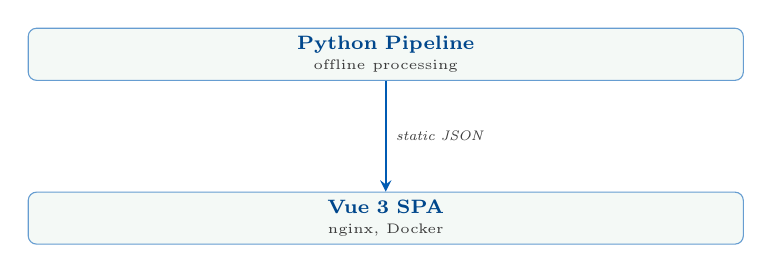
\begin{tikzpicture}[
  node distance=6pt,
  box/.style={
    draw=secondary!60, fill=lightbg, rounded corners=3pt,
    font=\scriptsize, inner xsep=5pt, inner ysep=3pt,
    text width=0.72\linewidth, align=center
  },
  arr/.style={->, >=stealth, thick, color=secondary}
]
  \node[box] (pipeline) {%
    \textbf{\color{primary}Python Pipeline}\\[-1pt]
    {\color{textgray}\tiny offline processing}};
  \node[box, below=40pt of pipeline] (spa) {%
    \textbf{\color{primary}Vue 3 SPA}\\[-1pt]
    {\color{textgray}\tiny nginx, Docker}};
  \draw[arr] (pipeline) -- node[right, font=\tiny\itshape, color=textgray] {static JSON} (spa);
\end{tikzpicture}
\end{center}

No backend at runtime — the SPA fetches pre-built JSON files.
Deployment via a single Docker Compose.

\vspace{2pt}
\sectiontitle{Interactive Map}

\includegraphics[width=\linewidth,height=5cm,keepaspectratio]{../images/europe_map.png}
\imgcap{Fig.\,1: Europe-wide view. Markers cluster automatically; green = IE member, blue = other.}

\columnbreak

%% ── COL 2 ──────────────────────────────────────────────────────────────────

\sectiontitle{Choropleth Layer}

Nine configurable combinations: \{BSc, MSc, PhD\} $\times$ \{enrolled, first-year, degrees\}
with four metrics — \emph{total}, \emph{female count}, \emph{female share (\%)}, \emph{per-million population}.

\includegraphics[width=\linewidth,height=4cm,keepaspectratio]{../images/color_map_female_10-11.png}
\imgcap{Fig.\,3: Female BSc count, 2010/11.}

\includegraphics[width=\linewidth,height=4cm,keepaspectratio]{../images/color_map_female_23-24.png}
\imgcap{Fig.\,4: Same metric, 2023/24. Absolute counts rose; relative shares barely moved.}

\vspace{2pt}
\sectiontitle{Statistical Charts}

\textbf{Enrollment Trends} — stacked bars separating first-year vs.\ returning cohorts for bachelor's level.

\includegraphics[width=\linewidth,height=4cm,keepaspectratio]{../images/enrollment_trends.png}
\imgcap{Fig.\,5: BSc enrollment, France. Dark = first-year; light = returning.}

\textbf{Female Representation} — dual line chart (BSc \& MSc) exposing persistent gender disparities at programme level.

\includegraphics[width=\linewidth,height=4cm,keepaspectratio]{../images/female_representation.png}
\imgcap{Fig.\,6: France BSc (blue) vs.\ MSc (orange) female share, 14 years. Both below 20\%.}

\columnbreak

%% ── COL 3 ──────────────────────────────────────────────────────────────────

\sectiontitle{European Context \& Density}

Three views: \textbf{Doughnut} (country shares), \textbf{Absolute Scale} (raw), \textbf{Density} (per million — small Nordic nations rank highest).

\includegraphics[width=\linewidth,height=4cm,keepaspectratio]{../images/eu_student_distribution.png}
\imgcap{Fig.\,6: France BSc (blue) vs.\ MSc (orange) female share, 14 years. Both below 20\%.}

\vspace{2pt}
\sectiontitle{Side-by-Side Comparison}

Any two countries or institutions can be placed in a \textbf{Compare} modal using \emph{colour hue} for degree levels and \emph{line style} (solid vs.\ dashed) to distinguish entities. Covers enrollment, degrees, and female share at BSc \& MSc level.

\includegraphics[width=\linewidth,height=5cm,keepaspectratio]{../images/student_enrollment_eter_comparison.png}
\imgcap{Fig.\,1: Europe-wide view. Markers cluster automatically; green = IE member, blue = other.}

\vspace{2pt}
\sectiontitle{Key Findings}

\begin{tightitem}
  \item Most European countries show \textbf{$<$25\% female share} at BSc level — nearly unchanged over 14 years
  \item Absolute female counts \emph{grew}, masking the stagnant relative share
  \item \textbf{Per-capita normalization shifts the picture}: small Nordic/Baltic nations rank highest once population size is accounted for
\end{tightitem}

\vspace{2pt}
\sectiontitle{Limitations \& Future Work}

\begin{tightitem}
  \item Manual pipeline re-run on each update; ETER may lag 2+ years
  \item Members-DATA = IE members only; fuzzy matching risk
\end{tightitem}

\textit{Future improvements:} CI/CD auto-refresh, choropleth animation, institution-type filter, mobile layout, CSV/PNG/PDF export.

\end{multicols}

\vspace{2pt}
{\color{primary}\rule{\linewidth}{0.8pt}}
{\centering\scriptsize\color{textgray}
KIV/VI --- Information Visualization $\cdot$
University of West Bohemia, Plze\v{n} $\cdot$ May 2026\par}

\end{document}